% Options for packages loaded elsewhere
\PassOptionsToPackage{unicode}{hyperref}
\PassOptionsToPackage{hyphens}{url}
%
\documentclass[
]{article}
\usepackage{amsmath,amssymb}
\usepackage{lmodern}
\usepackage{iftex}
\ifPDFTeX
  \usepackage[T1]{fontenc}
  \usepackage[utf8]{inputenc}
  \usepackage{textcomp} % provide euro and other symbols
\else % if luatex or xetex
  \usepackage{unicode-math}
  \defaultfontfeatures{Scale=MatchLowercase}
  \defaultfontfeatures[\rmfamily]{Ligatures=TeX,Scale=1}
\fi
% Use upquote if available, for straight quotes in verbatim environments
\IfFileExists{upquote.sty}{\usepackage{upquote}}{}
\IfFileExists{microtype.sty}{% use microtype if available
  \usepackage[]{microtype}
  \UseMicrotypeSet[protrusion]{basicmath} % disable protrusion for tt fonts
}{}
\makeatletter
\@ifundefined{KOMAClassName}{% if non-KOMA class
  \IfFileExists{parskip.sty}{%
    \usepackage{parskip}
  }{% else
    \setlength{\parindent}{0pt}
    \setlength{\parskip}{6pt plus 2pt minus 1pt}}
}{% if KOMA class
  \KOMAoptions{parskip=half}}
\makeatother
\usepackage{xcolor}
\IfFileExists{xurl.sty}{\usepackage{xurl}}{} % add URL line breaks if available
\IfFileExists{bookmark.sty}{\usepackage{bookmark}}{\usepackage{hyperref}}
\hypersetup{
  pdftitle={TAC\_report\_2022},
  pdfauthor={Fay},
  hidelinks,
  pdfcreator={LaTeX via pandoc}}
\urlstyle{same} % disable monospaced font for URLs
\usepackage[margin=1in]{geometry}
\usepackage{graphicx}
\makeatletter
\def\maxwidth{\ifdim\Gin@nat@width>\linewidth\linewidth\else\Gin@nat@width\fi}
\def\maxheight{\ifdim\Gin@nat@height>\textheight\textheight\else\Gin@nat@height\fi}
\makeatother
% Scale images if necessary, so that they will not overflow the page
% margins by default, and it is still possible to overwrite the defaults
% using explicit options in \includegraphics[width, height, ...]{}
\setkeys{Gin}{width=\maxwidth,height=\maxheight,keepaspectratio}
% Set default figure placement to htbp
\makeatletter
\def\fps@figure{htbp}
\makeatother
\setlength{\emergencystretch}{3em} % prevent overfull lines
\providecommand{\tightlist}{%
  \setlength{\itemsep}{0pt}\setlength{\parskip}{0pt}}
\setcounter{secnumdepth}{-\maxdimen} % remove section numbering
\newlength{\cslhangindent}
\setlength{\cslhangindent}{1.5em}
\newlength{\csllabelwidth}
\setlength{\csllabelwidth}{3em}
\newlength{\cslentryspacingunit} % times entry-spacing
\setlength{\cslentryspacingunit}{\parskip}
\newenvironment{CSLReferences}[2] % #1 hanging-ident, #2 entry spacing
 {% don't indent paragraphs
  \setlength{\parindent}{0pt}
  % turn on hanging indent if param 1 is 1
  \ifodd #1
  \let\oldpar\par
  \def\par{\hangindent=\cslhangindent\oldpar}
  \fi
  % set entry spacing
  \setlength{\parskip}{#2\cslentryspacingunit}
 }%
 {}
\usepackage{calc}
\newcommand{\CSLBlock}[1]{#1\hfill\break}
\newcommand{\CSLLeftMargin}[1]{\parbox[t]{\csllabelwidth}{#1}}
\newcommand{\CSLRightInline}[1]{\parbox[t]{\linewidth - \csllabelwidth}{#1}\break}
\newcommand{\CSLIndent}[1]{\hspace{\cslhangindent}#1}
\ifLuaTeX
  \usepackage{selnolig}  % disable illegal ligatures
\fi

\title{TAC\_report\_2022}
\author{Fay}
\date{2022-12-12}

\begin{document}
\maketitle

\hypertarget{abstract}{%
\section{Abstract}\label{abstract}}

Parasites in hybrid zones can give insight into species barriers, as
they are modulating the fitness of hybrid hosts. Recent findings have
demonstrated lower infection intensities with parasites in hybrids in
the European House Mouse Hybrid zone (HMHZ), indicating higher disease
resistance. However, tolerance has not yet been addressed in depth, as
it is impractical to measure in wild populations. In an attempt to
predict and evaluate the health impact of parasite infections and
extrapolate tolerance in the HMHZ, we use a machine learning method. A
random forest model was trained on immune parameters measured in
experimental lab infections with Eimeria and then applied to data
obtained from field sampling. Our predictions revealed that these
infections are more detrimental to hybrid male mice. This approach
represents an initial step in assessing tolerance in field studies.

\hypertarget{introduction}{%
\section{Introduction}\label{introduction}}

\hypertarget{methods}{%
\section{Methods}\label{methods}}

\hypertarget{mouse-strains-luke}{%
\subsubsection{Mouse strains (Luke)}\label{mouse-strains-luke}}

In order to gain a better understanding of tolerance in hybrid mice we
established a laboratory model of experimental lab infections with the
Eimeria spp. Our experimental setup is a variation of the framework in
Balard et al., 2020. The mice used are four wild-derived inbred mouse
strains and their generated F1 hybrids. The mouse strains are fully
inbred, as they have pased through at least 20 generations of sibling
pairing. From the fours strains, two were used as a representation of
the M. m. domesticus: SCHUNT (Locality: Schweben, Hessen, Germany {[}N:
5°0 26', E: 9°36'{]} Martincová et al. (2019)) and STRA (Locality:
Straas, Bavaria, Germany {[}N: 50°11', E: 11°46'{]} (Piálek et al.
(2008)). The two following strains were in turn derived from M. m.
musculus: BUSNA (Locality: Buškovice, Bohemia, Czech Republic {[}N: 5°0
14', E: 1°3 22'{]} (pialek2008development)) and PWD (Locality:
Kunratice, Bohemia, Czech Republic {[}N: 5°0 01', E: 14 2°9'{]}
(Gregorova, Forejt, et al. (2000)). In our setup there are two two
intersubspecific hybrids (STRAxBUSNA and SCHUNTxPWD) and two
intrasubspecific hybrids (SCHUNTxSTRA and PWDxBUSNA). The mice were
between 5.6 and 21.4 weeks. The mice were acquired from the Institute of
Vertebrate Biology of the Czech Academy of Sciences in Studenec (license
number 61974/2017-MZE-17214; for further details on strains see
\url{https://housemice.cz/en}).

Infections with the parasite Eimeria induce a protective immune reaction
in the host against reinfection (Rose et al., 1992a; Smith \& Hayday,
2000). The feces of the naive mice were tested to ensure that the mice
were Eimeria spp., prior to infection, following the methods of Balard
Balard, Jarquı́n-Dı́az, Jost, Mittné, et al. (2020).

\hypertarget{infections-with-eimeria-spp.-luke}{%
\subsubsection{Infections with Eimeria spp.
(Luke)}\label{infections-with-eimeria-spp.-luke}}

The procedure used is as described in in Balard et al., 2020. During the
infections mice were housed solo in cages. We infected the mice orally
with 150 sporulated oocysts of one Eimeria isolate suspended in 100 µl
phosphate-buffered saline (PBS). The mice had access to food and water
ad libitum SNIFF, Rat/Mouse maintenance feed 10 mm and were observed
daily for 8 days until their sacrifice by cervical dislocation. In the
case that individual mice showed severe adverse health effects or
extreme weigh loss of more than 18\% relative to their weight at the
start of experiment, were then sacrificed earlier at defined humane end
points (experiment license Reg. 0431/17). Daily measurements of weight
were recorded and fecal matter was gathered. Collected feces were
supspended in 2\% potassium dichromate and paaracite oocysts were
retrieved by NaCl flotation.

To enable a consistent distribution between experimental groups, mice
were allocated at random, while ensuring a similar distribution of age
and sex between groups.

\hypertarget{gene-expression-high-thoughput-qpcr-luke}{%
\subsubsection{Gene expression high-thoughput qPCR
(Luke)}\label{gene-expression-high-thoughput-qpcr-luke}}

Homogenized caecum tissue was processed for RNA using the filter based
innuPREP RNA Mini Kit 2.0 (Jena analytik, Germany) according to
manufacturer instructions. Extracted RNA was quantified using NanoDrop
2000c (Thermo Scientific, Waltham, USA) and transcribed into cDNA with
iScript (Bio-rad Laboratories, Hercules, California, United States),
following manufacturer protocol. Gene expression was ascertained via
hight-throughput qPCR of cDNA from the caecum extracted material, plated
onto Fluidigm IFC (integrated fluidic circuit), initialized by the Juno
controller and read in the Fluidigm BioMark HD (PN 100-7222 C1,
Fluidigm, South San Francisco, California, United States). After cDNA
conversion mentioned above, the samples went through the recommended
preparation steps, carried out in sterile extractor hood, with reagents
being kept at 4 °C when in use, and at -20 °C when stored overnight. All
pipetting was done using sterile filter tips. Table of wet-lab tested
primers can be found in the appendix file 20614FDGP21T1\_DESIGN

\hypertarget{specific-target-amplification-sta-using-fluidigm-preamp-master-mix-luke}{%
\subsubsection{Specific target amplification (STA) using Fluidigm PreAmp
master mix
(Luke)}\label{specific-target-amplification-sta-using-fluidigm-preamp-master-mix-luke}}

ll primers at 100µM were pooled together in a micro centrifuge tube and
resulting solution was diluted to a final concentration of 500 nM, with
a 10 mM Tris-HCl (pH 8,0), 0.1 mM EDTA TE Buffer (12090-015, Invitrogen,
Waltham, Massachusetts, United States). Fluidigm Preamp Master Mix
(Fluidigm PN 100-5580) was added to the solution according to the
manufacturer instructions, to create delta gene assay Preamp Master Mix.
Sample cDNA (including a non-template control (NTC)) was plated onto
96-well plates and the master mix added to each well. Sample plate was
then gently vortexed for 5 seconds and spun down at 1,000 x g for 1
minute. The amplification reactions were carried out in the Biometra
TOne 96 (846-2-070-301, Analytic Jena, Jena, Germany) at the following
cycling conditions: Hold at 95 ºC for 2 minutes, 95 ºC for 15 seconds,
then 60 ºC for 4 minutes (15x), Hold at 4 ºC for infinity.

\hypertarget{primers-and-sample-preparation-luke}{%
\subsubsection{Primers and sample preparation:
(Luke)}\label{primers-and-sample-preparation-luke}}

1.5 µL of primer (wet lab tested) at 100 µM ,13.5 µL of TE Buffer and 15
µL of 2X Assay Loading Reagent (PN 100-7611, Fluidigm), were combined to
create 10X Assay solutions. Sample reaction mixes were then created by
combining 1.8 µL of preamplified and Exonuclease I treated cDNA, 2 µL of
2X SsoFast EvaGreen Supermix with low ROX™ (Bio-Rad, PN 172-5211) and
192.24 Delta Gene Sample Reagent (PN 100-6653, Fluidigm), to create 4 µL
stock per 1 sample reaction. This was scaled to accommodate sample
repeat runs. Prepared samples and primers were stored at -20°C until the
IFC chips were primed.

\hypertarget{ifc-qpcr-runs-luke}{%
\subsubsection{IFC qPCR runs (Luke)}\label{ifc-qpcr-runs-luke}}

The 192.24 IFC was plated and treated as per manufacturer instructions
(PN 100-7222 C1), consisting of control line fluid injection into
accumulator 2 slot, removal of protective film, pipetting of samples and
10X assay mixes in 3 µL volumes, adding 150 µL of Actuation Fluid (PN
100-6250) into the P1 port, 150 µL of Pressure Fluid (PN 100-6249) into
the P2 and P3 ports, 20 µL of Pressure Fluid into the P4 and P5 ports
and finally initializing the IFC in the Juno controller, using the Load
Mix 192.24 GE script. After the initialization completed, the IFC was
transferred into the BioMark HD and the assay properties were set as
follows: Application type: Gene Expression, Passive reference: ROX,
Assay: Single probe, Probe type: EvaGreen, using the GE 192x24 PCR+Melt
v2.pcl protocol, on Auto-exposure.

\hypertarget{wild-mice}{%
\subsection{Wild mice}\label{wild-mice}}

During the years 2016 to 2019, we sampled 1889 mice in the House Mouse
Hybrid zone. We used live traps to capture mice in farms and houses,
during September every year. To catch mice of \emph{M. musculus
musculus}, \emph{M. musculus domesticus} and hybrid origin, we selected
a large geographic area in Brandenburg and Neuruppin. For each mouse, we
have collected information during dissections, on their body length,
their weight and their pathophysiology. Tissue samples were used to
genotype the hosts. Further information on the set-up of the experiment
can be found in previous publications of the group Balard, Jarquı́n-Dı́az,
Jost, Martincová, et al. (2020) From 1889 mice, 336 were selected with a
varying genotype for Fluidigm BioMark assay. Another 95 were selected
for fluorescence-activated cell sorting.

\hypertarget{statistical-analysis}{%
\subsection{Statistical Analysis}\label{statistical-analysis}}

\hypertarget{imputation-of-missing-data}{%
\subsubsection{Imputation of missing
data}\label{imputation-of-missing-data}}

To make the most of our data collection, we aimed to resolve
missingness. Missing data were imputed using multiple imputations by
chained equations. We used the package MICE in R Van Buuren and
Groothuis-Oudshoorn (2011), with five imputed data sets and five
iterations. Data generated by FACS or the Gene Expression / Biomarker
assay were regarded as missing if each mouse had measurements for some
variables. For each continuous variable, we specified a predictive mean
matching model. All the remaining variables were used as predictors in
the imputation. To control the quality of our imputations, we evaluated
the distribution plot of the existing data and the imputed data for all
measurements \ref{fig:fig1} \ref{fig:fig2}. Further, we tested for
convergence. We assume data is ``missing completely at random'' or
``missing at random''. For both types of missingness, multiple
imputation is a suggested method to impute missing variables Van Buuren
(2018).

\begin{figure*}[th]
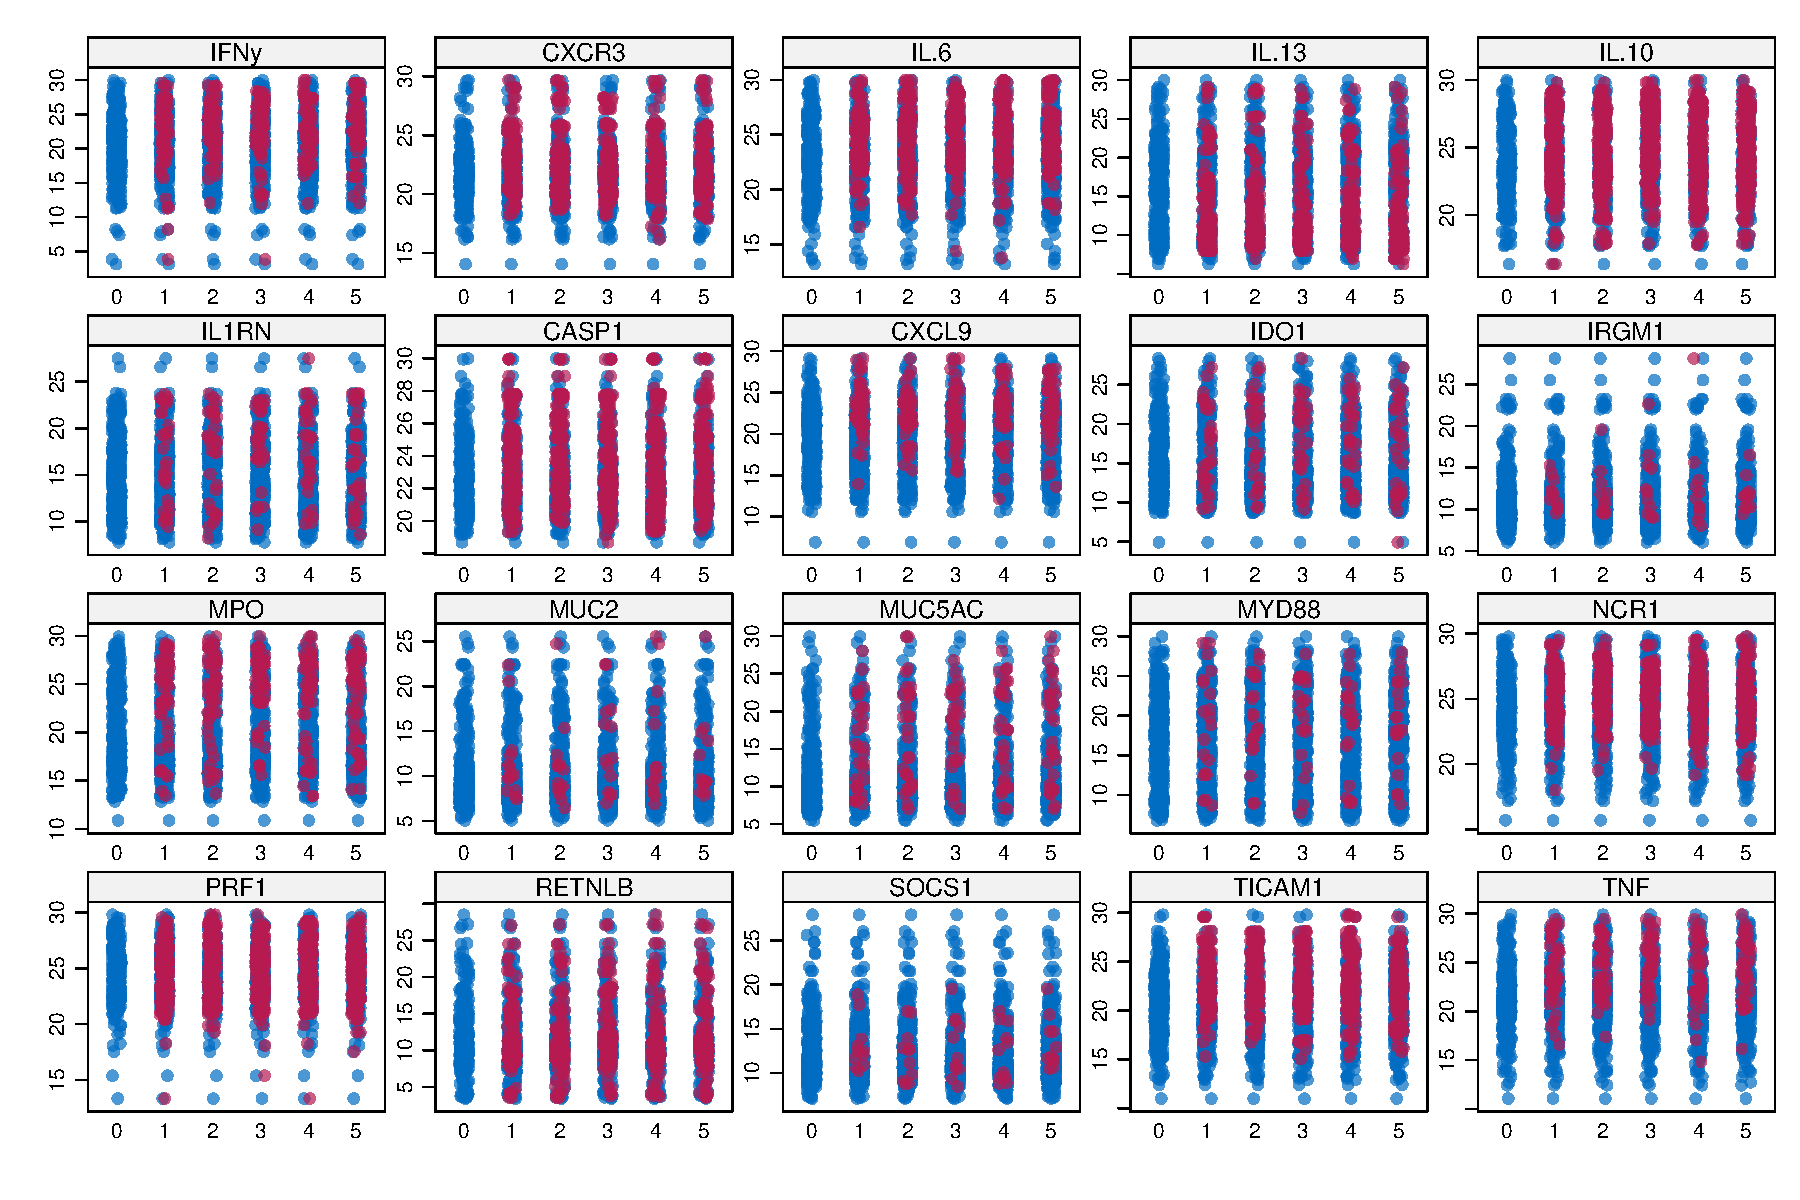
\includegraphics[width=1\linewidth]{TAC_report_2022_files/figure-latex/fig1-1} \caption{Stripplot of observed and imputed data}\label{fig:fig1}
\end{figure*}

\begin{figure*}[th]
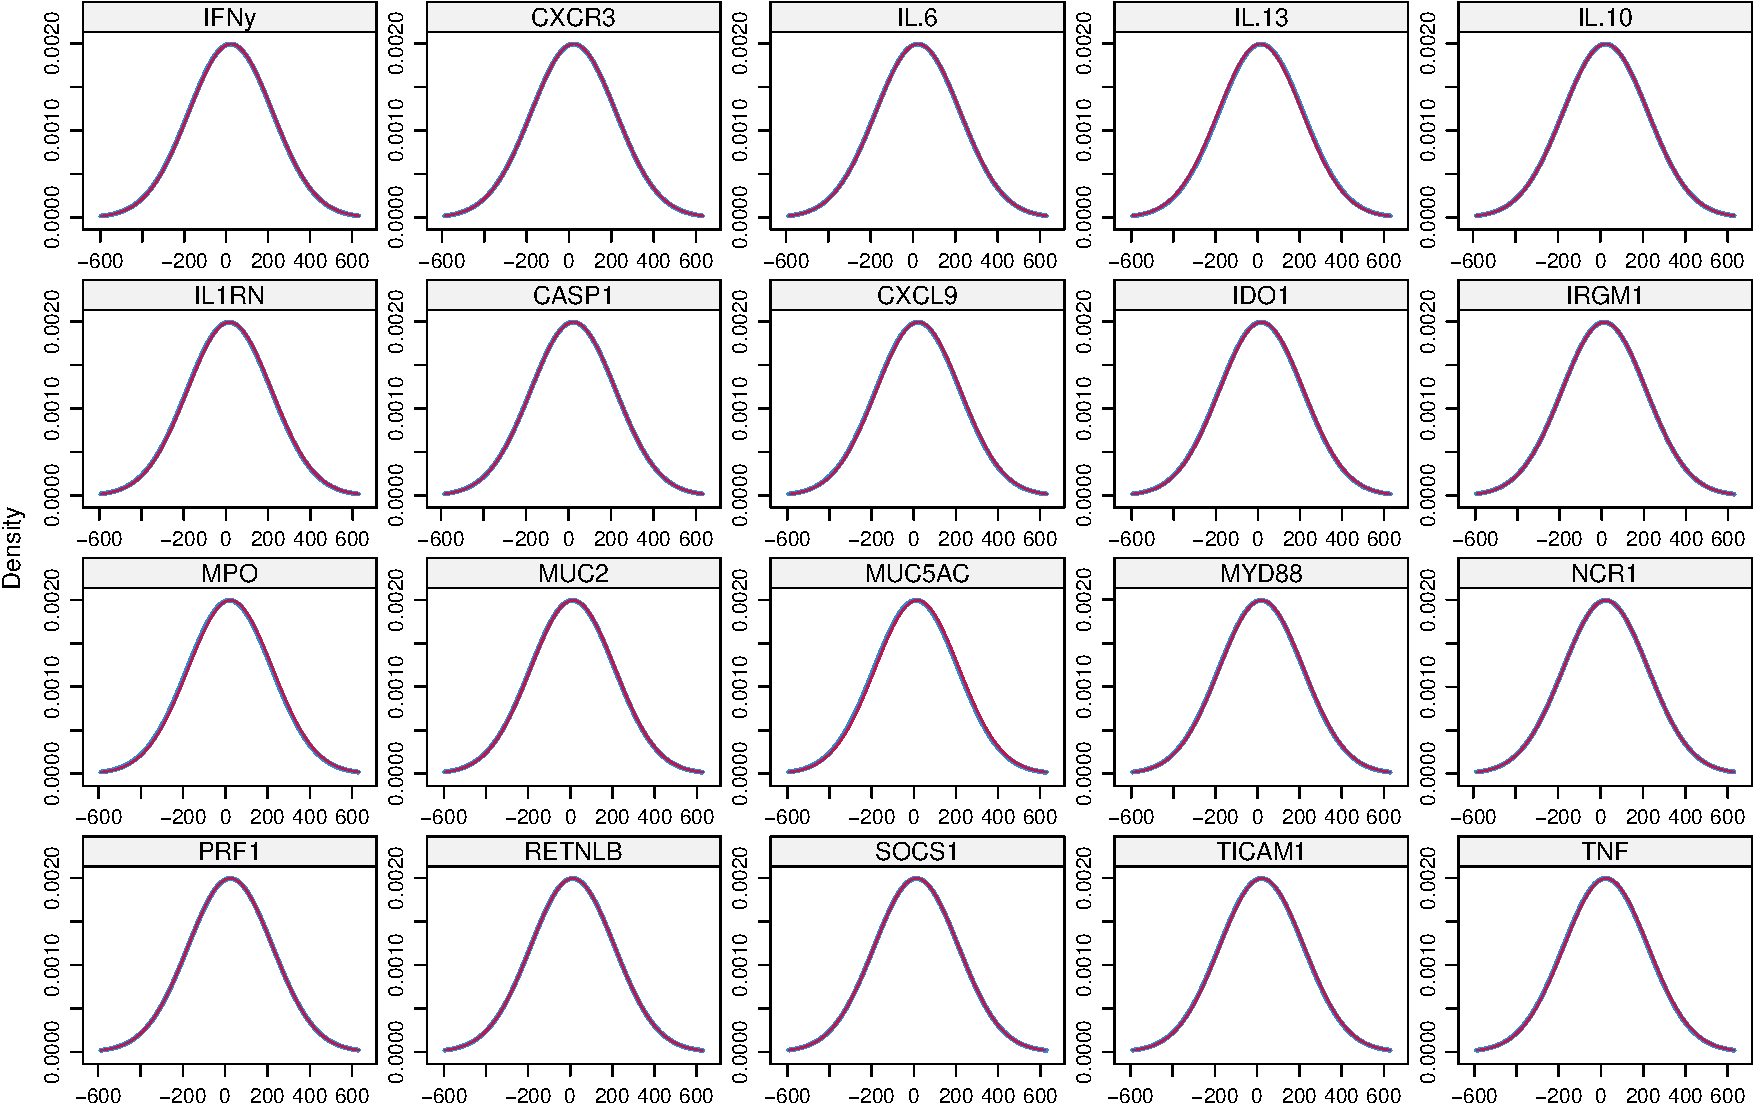
\includegraphics[width=1\linewidth]{TAC_report_2022_files/figure-latex/fig2-1} \caption{Density plot of observed and imputed data}\label{fig:fig2}
\end{figure*}

\hypertarget{questions-to-dos}{%
\paragraph{Questions / To-dos:}\label{questions-to-dos}}

\begin{enumerate}
\def\labelenumi{\arabic{enumi}.}
\tightlist
\item
  Should I log-transform the data prior to imputation?
\item
  Increasing produced data sets / iterations
\item
  sensitivity analyses using complete cases only
\end{enumerate}

\hypertarget{random-forest}{%
\subsubsection{Random forest}\label{random-forest}}

In an attempt to predict the health impact of infections in mice, we
used a random forest model Breiman (2001). We chose the maximum weight
loss during the experimental laboratory infections of mice with the
parasite \emph{Eimeria spp.} as a response variable. Maximum weight loss
is here used as a proxy describing the health impact caused by
infections. The random forest was constructed utilizing the expression
data of 20 genes, obtained by the biomarker assay (utilizing the R
package ``randomForest,'' ntree = 1000). The data set was split into a
training data set of 70 \% and to a testing data set of 30 \% to avoid
over-fitting and to assess the performance of the model on ``unseen''
data.

As a quality assessment, we used k- fold cross validation, where the
data set is divided into k subsets. Each time, the model is assessed by
using one of the k subsets as the test data set and the other as the
training data set. The model was then fitted on each k-subset and
afterwards evaluated on the test set. Last the evaluation score was
noted and the model then discarded. Further, a permutation test
cross-validation was implemented (using the function
``rf.crossValidation'' (using the R package rfUtilities, version 2.1-5).
The percent variance explained from the specified fit model was 27.7\%.
Moreover, the mean squared error from each bootstrapped model was 44.14.
Next, the variable importance was calculated according to the total
decrease in node impurities from splitting on each variable, averaged
over all trees. In this case of regression, the node impurity is
measured by residual sum of squares. Variables with comparatively higher
importance have a greater impact on the predictions of the model.

\begin{verbatim}
## running: regression cross-validation with 99 iterations
\end{verbatim}

\begin{verbatim}
## [1] 27.7
\end{verbatim}

\begin{verbatim}
## [1] 44.13772
\end{verbatim}

\begin{verbatim}
## [1] 78
\end{verbatim}

\begin{verbatim}
## [1] 6.543936
\end{verbatim}

\begin{figure*}[th]
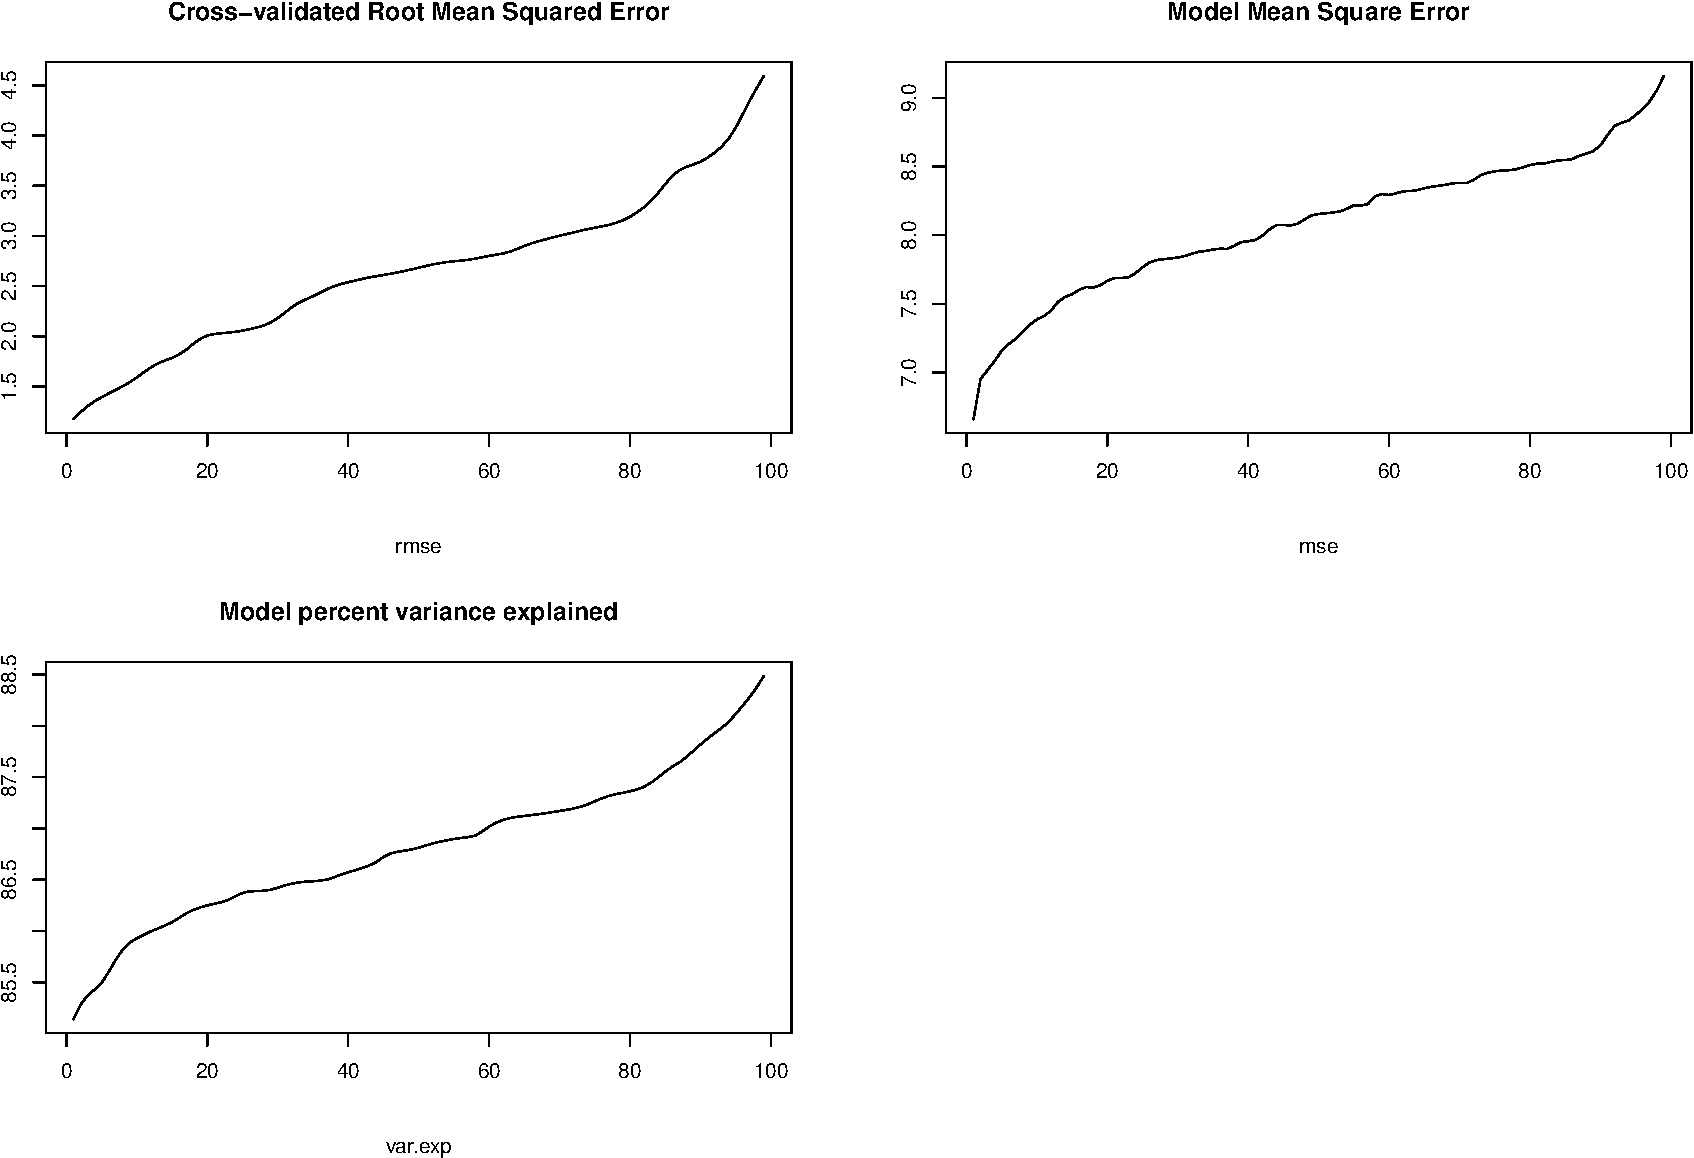
\includegraphics[width=1\linewidth]{TAC_report_2022_files/figure-latex/fig4-1} \caption{Variance explained and Root Mean Squared Error}\label{fig:fig4}
\end{figure*}

\begin{verbatim}
##        IncNodePurity Var.Names
## SOCS1       582.5419     SOCS1
## TICAM1      549.4166    TICAM1
## CXCL9       538.1206     CXCL9
## IL.6        459.0768      IL.6
## IFNy        395.9684      IFNy
## IL1RN       327.9611     IL1RN
## RETNLB      289.5686    RETNLB
## NCR1        239.8289      NCR1
## TNF         226.3735       TNF
## MPO         214.1609       MPO
## IL.13       201.9333     IL.13
## MUC2        200.2868      MUC2
## MYD88       196.5789     MYD88
## IRGM1       178.2120     IRGM1
## CASP1       170.0408     CASP1
## CXCR3       169.9418     CXCR3
## IDO1        162.3620      IDO1
## PRF1        161.2846      PRF1
## IL.10       156.3871     IL.10
## MUC5AC      149.1062    MUC5AC
\end{verbatim}

\begin{figure*}[th]
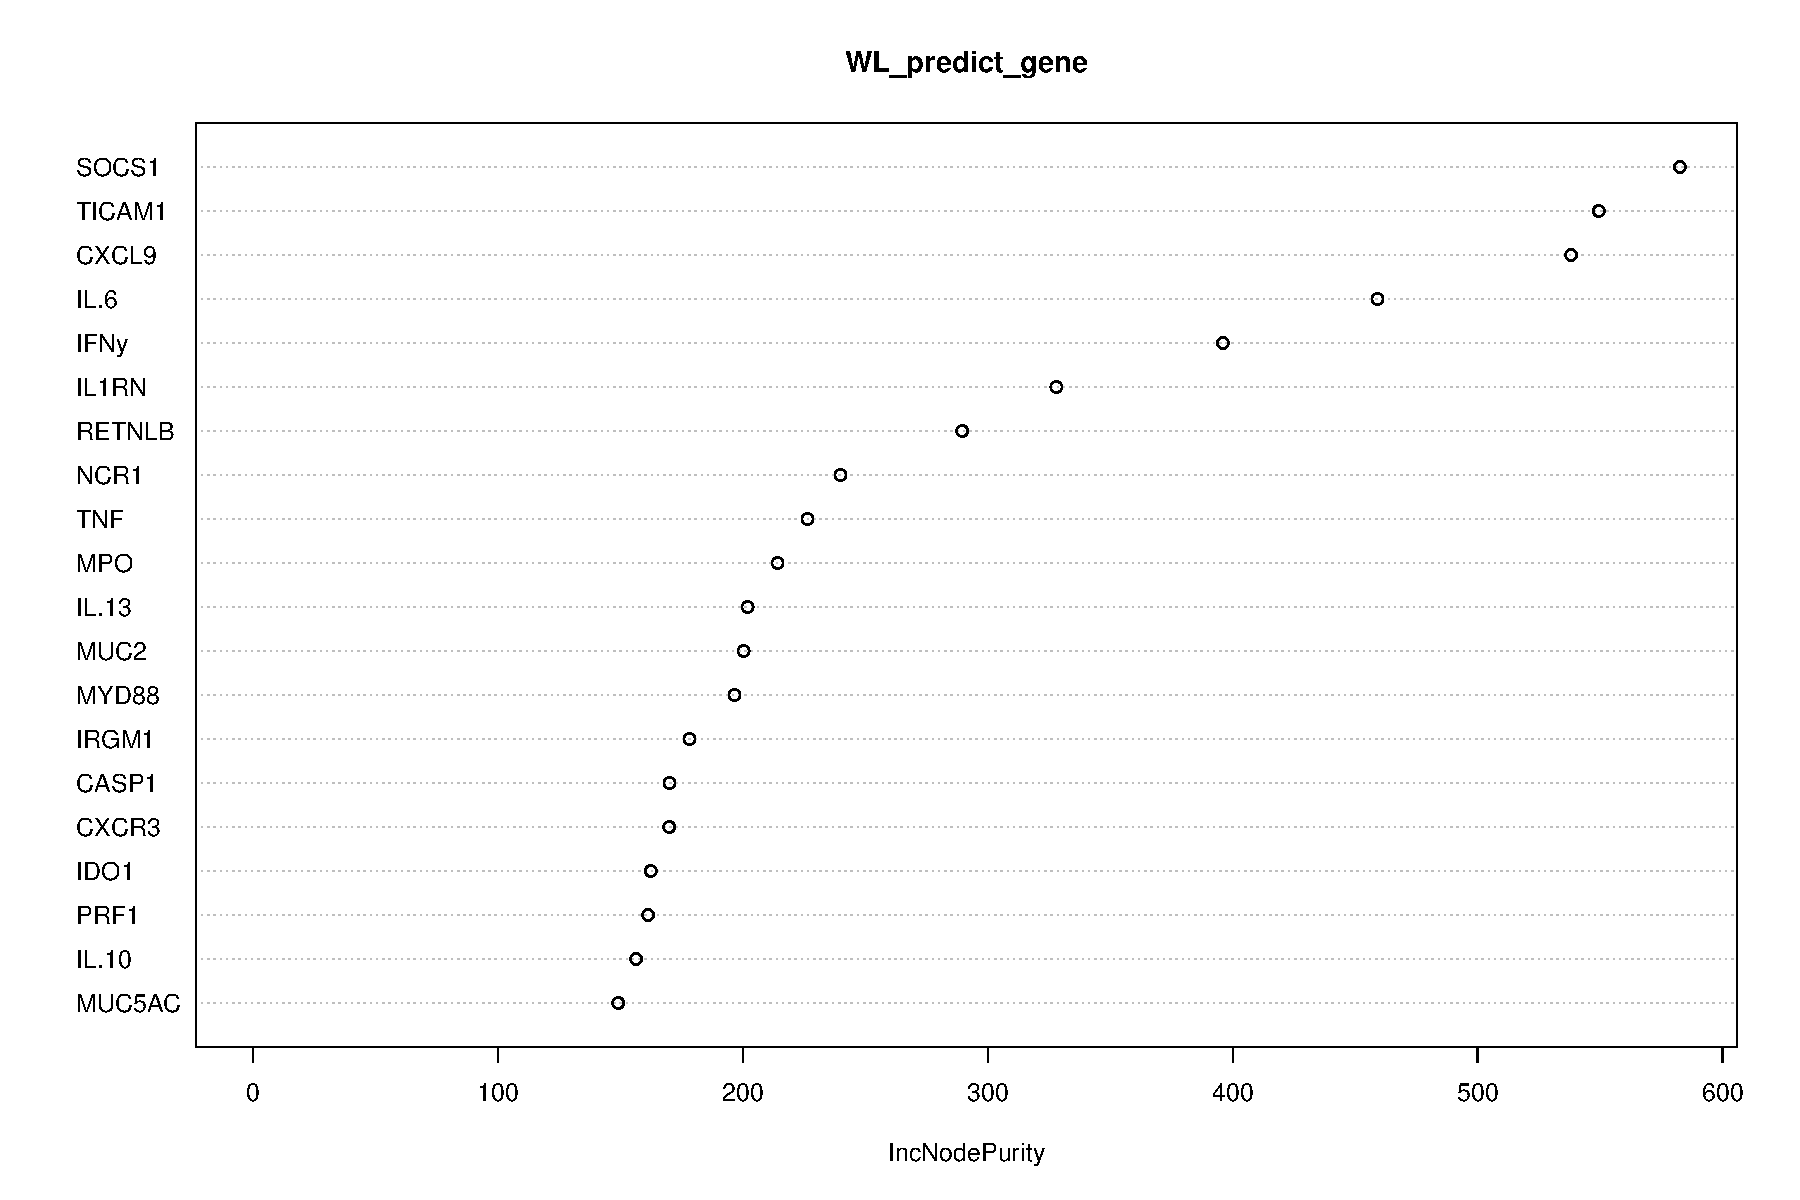
\includegraphics[width=1\linewidth]{TAC_report_2022_files/figure-latex/fig6-1} \end{figure*}

\hypertarget{results}{%
\section{Results}\label{results}}

\hypertarget{discussion}{%
\section{Discussion}\label{discussion}}

\hypertarget{conclusion}{%
\section{Conclusion}\label{conclusion}}

\hypertarget{literature-citations}{%
\section{Literature citations}\label{literature-citations}}

\hypertarget{references}{%
\section*{References}\label{references}}
\addcontentsline{toc}{section}{References}

\hypertarget{refs}{}
\begin{CSLReferences}{1}{0}
\leavevmode\vadjust pre{\hypertarget{ref-balard2020intensity}{}}%
Balard, Alice, Vı́ctor Hugo Jarquı́n-Dı́az, Jenny Jost, Iva Martincová,
L'udovı́t Ďureje, Jaroslav Piálek, Miloš Macholán, Joëlle Goüy de
Bellocq, Stuart JE Baird, and Emanuel Heitlinger. 2020. {``Intensity of
Infection with Intracellular Eimeria Spp. And Pinworms Is Reduced in
Hybrid Mice Compared to Parental Subspecies.''} \emph{Journal of
Evolutionary Biology} 33 (4): 435--48.

\leavevmode\vadjust pre{\hypertarget{ref-balard2020coupling}{}}%
Balard, Alice, Vı́ctor Hugo Jarquı́n-Dı́az, Jenny Jost, Vivian Mittné,
Francisca Böhning, L'udovı́t Ďureje, Jaroslav Piálek, and Emanuel
Heitlinger. 2020. {``Coupling Between Tolerance and Resistance for Two
Related Eimeria Parasite Species.''} \emph{Ecology and Evolution} 10
(24): 13938--48.

\leavevmode\vadjust pre{\hypertarget{ref-breiman2001random}{}}%
Breiman, Leo. 2001. {``Random Forests.''} \emph{Machine Learning} 45
(1): 5--32.

\leavevmode\vadjust pre{\hypertarget{ref-gregorova2000pwd}{}}%
Gregorova, S, J Forejt, et al. 2000. {``PWD/Ph and PWK/Ph Inbred Mouse
Strains of Mus m. Musculus Subspecies--a Valuable Resource of Phenotypic
Variations and Genomic Polymorphisms.''} \emph{Folia Biol (Praha)} 46
(1): 31--41.

\leavevmode\vadjust pre{\hypertarget{ref-martincova2019phenotypic}{}}%
Martincová, Iva, L'udovı́t Ďureje, Jakub Kreisinger, Miloš Macholán, and
Jaroslav Piálek. 2019. {``Phenotypic Effects of the y Chromosome Are
Variable and Structured in Hybrids Among House Mouse Recombinant
Lines.''} \emph{Ecology and Evolution} 9 (10): 6124--37.

\leavevmode\vadjust pre{\hypertarget{ref-pialek2008development}{}}%
Piálek, Jaroslav, Martina Vyskočilová, Barbora Bı́mová, Dana Havelková,
Jana Piálková, Petra Dufková, Věra Bencová, et al. 2008. {``Development
of Unique House Mouse Resources Suitable for Evolutionary Studies of
Speciation.''} \emph{Journal of Heredity} 99 (1): 34--44.

\leavevmode\vadjust pre{\hypertarget{ref-van2018flexible}{}}%
Van Buuren, Stef. 2018. \emph{Flexible Imputation of Missing Data}. CRC
press.

\leavevmode\vadjust pre{\hypertarget{ref-van2011mice}{}}%
Van Buuren, Stef, and Karin Groothuis-Oudshoorn. 2011. {``Mice:
Multivariate Imputation by Chained Equations in r.''} \emph{Journal of
Statistical Software} 45: 1--67.

\end{CSLReferences}

\end{document}
